\bigbreak
%\section*{Introduction}
\lettrine{A}{s} described and illustrated in the previous chapter, a fundamental limitation of Surprise lies in its definition in terms of discrete probability and binomial coefficients that make it applicable only to binary networks, i.e. graphs with edge values $1$ or $0$.
This represents a substantial drawback, for it requires binarization of brain connectivity networks, thus discarding potentially important information contained in the edge weight distribution.
Moreover, different binarization procedures may lead to different network representations for the same connectivity dataset.
Therefore, an extension of Surprise to weighted networks would be highly desirable, and would provide a new and important tool to study the modular organization of brain connectivity beyond the resolution limit.

Capitalizing on recent development in the field of statistical physics of complex networks~\cite{traag2015}, in this chapter we describe and demonstrate the use of Asymptotical Surprise, a weighted counterpart to Surprise, in the study of the modular structure of weighted networks.
Moreover, we propose a new algorithm, dubbed PACO (PArtitioning Cost Optimization) for the maximization of Asymptotical Surprise, that has its roots in the previously described FAGSO algorithm.

Since there is no ground-truth structure for brain functional connectivity networks, we have assessed the performance of this novel approach on synthetic networks with a planted modular structures, and compared it to some of the leading graph partitioning methods.
Importantly, we demonstrate our approach in networks  derived from synthetic data that mimic different structures, levels of noise and variability, such as those observed in functional connectivity experimental data.
Indeed, improved resolution afforded by Asymptotical Surprise may imply increased vulnerability to spurious modules resulting from noisy correlations.
It is therefore important to assess the benefits of increased resolution against the limitations arising from intrinsic data variability. 

Finally, we apply Asymptotical Surprise to weighted functional connectivity networks from resting state fMRI data, revealing a heterogeneous, multiscale community structure. We show that the finer modular subdivision of resting state functional connectivity networks obtained by Asymptotical Surprise leads to substantial differences in the identification of connector hubs compared to other community detection methods.

\section{Asymptotical Surprise}
As introduced in the previous sections, Surprise~\cite{aldecoa2011,aldecoa2013} is a quality measure of the partition of a binary network that has its roots in probability theory.
For a given partition $\zeta$, Surprise represents the probability that a graph drawn uniformly at random from the set of all graphs with $n$ nodes, $p=\binom{n}{2}$ pairs and $m$ edges has at least as many intra-cluster edges as $G$. Intuitively the lower the probability the better the partition.  For binary networks, Surprise can be computed within the discrete probability theory of urn models as shown in Equation~\ref{eq:surprise}.

In developing a quality function inspired to the principle of Surprise that works for weighted networks, it's convenient to consider the asymptotical expansion of the hypergeometric distribution. We introduce  $q=m_\zeta/m$ and $\left<q \right>=p_\zeta/p$ as the observed and expected fraction of intracluster edges. By only taking into account the dominant term of the sum in Eq.~\ref{eq:surprise} (the one with $i=m_\zeta$), we obtain with some manipulations an approximate expression for the logarithmic of Surprise:
\begin{equation}\label{eq:surprise_dominant}
\log(S) \approx \log \left( \frac{\binom{\left<q\right> p}{m_\zeta} \binom{(1-\left<q\right>)p}{m(1-q)}}{\binom{p}{m}} \right)
\end{equation}
which corresponds to the probability of observing exactly $m_\zeta$ internal links, given the clustering $\zeta$. As the denominator in Eq.\ref{eq:surprise_dominant} is independent of the partition, we ignore it, and thanks to the Stirling approximation of the binomial coefficients, which reads 
\begin{equation}
\log \binom{n}{k} \approx k \log \left( \frac{n}{k} \right)
\end{equation}
we can write this last dominant term~\ref{eq:surprise_dominant} as:
\begin{equation}
\log(S) = - \log \left(\frac{m}{p}\right)^{-m} \left[ \left(\frac{\left< q\right>}{q}\right)^q \left(\frac{1-\left< q\right>}{1-q}\right)^{1-q} \right]^{m}
\end{equation}
Discarding the term $(m/p)^{-m}$, independent of the partition, we obtain an asymptotic expansion of Surprise that reads:
\begin{equation}
\log(S) = -m \left[ q \log \frac{\left<q\right>}{q} + (1-q)\log \frac{1-\left<q\right>}{1-q} \right]
\end{equation}
Interestingly, this last equation corresponds to the binary Kullback-Leibler divergence $m D_{KL}(q \| \left< q \right>)$, which is interpretable as the distance between the two probability distributions $q$ and $\left<q\right>$, or more precisely, as the information lost (in nats since we are using natural base logarithms) when we encode the distribution $q$ with the distribution $\left< q\right>$. 
Thus, in the limit of large networks, Surprise $\hat{S}$ can be approximated by a binomial distribution: this observation led to definition of Asymptotical Surprise $\mathcal{S}_a$~\cite{traag2015}:

\begin{equation}\label{eq:asymptoticalsurprise}
\mathcal{S}_a = m D_{\textrm{KL}}\left( q \| \left< q \right> \right)
\end{equation}

where the binary Kullback-Leibler divergence~\cite{kullback1951} is $$D_{\textrm{KL}}(x\|| y) = x \log \left(\frac{x}{y} \right) + (1-x)\log \left (\frac{1-x}{1-y} \right).$$

In the framework of information theory~\cite{cover2006}, Asymptotical Surprise represents the Kullback-Leibler divergence between the observed and expected fraction of intra-cluster edges; it encodes the information lost when the prior distribution $\left <q \right >$ is used to approximate the posterior distribution $q$. Kullback-Leibler divergence is a quasi-distance on probability distributions as it is always non-negative, non-symmetric and zero only when $q=\left< q \right>$, like binary Surprise.

Asymptotical Surprise has a simpler formulation than binary Surprise as there are no binomial coefficients to evaluate and it has been shown to be resolution-limit-free in the limit of large networks ~\cite{traag2015}. Nicely, Asymptotical Surprise transparently allows the extension of Surprise to weighted networks, when the intracluster density consider edge weights. This powerful property made Asymptotical Surprise suited for community detection in weighted networks and in particular to brain functional connectivity networks, seamlessly permitting the need of sparsification procedures prior to the community detection, as shown in~\cite{nicolini2017}.

Numerically Asymptotical Surprise approximates very well Surprise already for networks with more than 50 nodes, as shown in Figure~\ref{fig:asymptotical_surprise_comparison}.

\begin{figure}[htb!]
\centering
\includegraphics[width=0.8\textwidth]{images/asymptotical_surprise_comparison.pdf}
\caption{Approximation of binary Surprise with a binomial formulation and the Asymptotical formulation based on the Kullback-Leibler divergence. In the inset, the approximation ratio of binomial and Asymptotical Surprise to hypergeometric Surprise tends to 1 for graphs larger than 50 nodes. Adapted from~\cite{traag2015}.}
\label{fig:asymptotical_surprise_comparison}
\end{figure}


\subsection{Maximization of Asymptotical Surprise}
Finding the optimal partition of a graph is an NP-hard problem~\cite{fortunato2010} and practical implementations of community detection rely on heuristic approaches that enable finding nearly-optimal solutions in a reasonable computation time.

Here we introduce a powerful and general method for the optimization of Asymptotical Surprise dubbed PACO (PArtitioning Cost Optimization). PACO is a non-deterministic agglomerative algorithm based on FAGSO (described in chapter~\ref{sec:max_surprise_fagso}) and, like the Louvain method, has an element of randomness that enables a more efficient exploration of the partition landscape.

The operating principle of PACO is based on the triadic closure property, i.e. the fact that in real-world networks nodes with many common neighbors are more likely to be neighbors. This transitive neighborhood property underlies the formation of communities of nodes~\cite{bianconi2014,eustace2015}. In principle, any measure of structural similarity between nodes could guide a community detection heuristic toward the optimal partition. Specifically, PACO uses the Jaccard index~\cite{jaccard1901}, a measure of the fraction of overlap between the neighbors in common between nodes, as the guiding principle for the agglomeration of similar nodes in the same community.

In the first phase of PACO, the Jaccard metric is evaluated for every edge. More formally, for an edge $e=(u,v)$ the Jaccard index is computed as $J(e)=\frac{|\Gamma(u) \cap \Gamma(v)|}{|\Gamma(u) \cup \Gamma(v)|}$ where $\Gamma(u)$ and $\Gamma(v)$ are the neighboring nodes of $u$ and $v$ respectively.

The agglomerative process starts with an initial partition where every vertex represents a community on its own. This partition has $n$ communities and no intra-cluster edges.
The edges of the graph are then ranked in decreasing order by their Jaccard index and iteratively, for every edge in the sorted list, endpoint nodes are merged only if they belong to different communities. In this case one of the two endpoints, selected by chance, is assigned to the other's endpoint community and the increment of Surprise is computed: if it is positive, the partition is updated together with the new value of Surprise (or Asymptotical Surprise), otherwise the algorithm proceeds to the next edge.  

Figure~\ref{algo:paco} describes the details of the PACO algorithm for Surprise and Asymptotical Surprise Optimization.
The function \textsc{Paco} takes as input a graph G and returns the nodes community membership vector C. Line 1 initializes the value of Surprise to 0. Line 2 assign to each node in the graph its community. Line 3 creates a list of edges E' sorted in decreasing order by their Jaccard coefficient. Line 4 iterates on every edge e=(u,v) and at line 6 checks if the endpoints they share the same community. Line 8 copies the membership vector to a temporary vector C'. Lines 9-13 choose randomly at chance if to put node u in the community of v or viceversa. Line 14 computes the new value of Surprise S' from the just updated community membership C. The function \textsc{ComputeSurprise} returns the value of Surprise for graph G and partition C. Lines 15 to 18 checks if the new value of Surprise S' is greater than the previously stored value S and update Surprise and the membership vector, otherwise continue to the next edge. Line 19 returns the final community membership assignment.

%%%% PACO %%%%
\begin{Algorithm}[htb!]
\begin{codebox}
\Procname{$\proc{Paco}(G)$}
\li $S\gets 0$ \Comment \emph{Initialize Surprise to $0$}
\li $C \gets (1,\ldots,|V|)$  \Comment \emph{Initialize membership vector}

% \End
\li $E' \gets \proc{Sort-Jaccard}(E)$ \Comment \emph{Sort edges in decreasing order by Jaccard index}

\li \For each edge $(u,v)$ in $E'$
\li \Do \li \If $C[u] \neq C[v]$ \Comment \emph{try to move nodes only if in different communities}
\li \Then
\li $C' \gets C$ \Comment \emph{Create a temporary membership vector}
\li \If \proc{UnifRand(0,1)} $< 0.5$ 
\li \Then 
\li $C'[v] \gets C[u]$
\li	\Else
\li $C'[u] \gets C[v]$ \End
\li $S' =$ \proc{ComputeSurprise($G$,$C'$)}
\li \Do \If $S'>S$
\li \Then
\li $C \gets C'$ \Comment \emph{update membership}
\li $S' \gets S$ \Comment \emph{update Surprise}
\End
\End \End \End
\li \Return $C$
\end{codebox}
\caption{Pseudocode of the PACO algorithm. The function PACO takes as input a graph $G$ and returns the nodes community membership vector $C$. Line $1$ initializes the value of Surprise to $0$. Line $2$ assign to each node in the graph its community. Line $3$ creates a list of edges $E'$ sorted in decreasing order by their Jaccard coefficient. Line $4$ iterates on every edge $e=(u,v)$ and at line $6$ checks if the endpoints they share the same community. Line $8$ copies the membership vector to a temporary vector $C'$. Lines $9-13$ choose randomly at chance if to put node $u$ in the community of $v$ or viceversa. Line $14$ computes the new value of Surprise $S'$ from the just updated community membership $C$. The function \textsc{ComputeSurprise} returns the value of Surprise for graph $G$ and partition $C$. Lines $15$ to $18$ checks if the new value of Surprise $S'$ is greater than the previously stored value $S$ and update Surprise and the membership vector, otherwise continue to the next edge. Line $19$ returns the final community membership assignment.}
\label{algo:paco}
\end{Algorithm}

The running time of PACO is linear in the number of nodes and quadratic in the average degree of the network, as shown 


\subsection{Comparison of PACO and FAGSO}

FAGSO is an agglomerative optimization algorithm that builds on a variation of the Kruskal algorithm for minimum spanning tree and is described in~\cite{nicolini2016}. The first step of this method consists in ranking the edges in the graph in decreasing order by the Jaccard index of the neighbors of their two endpoints vertices. An union-find data structure is used to hold the community structure throughout the computation. At the beginning, each community consists only of one vertex. Then, starting from the edge with the highest Jaccard index at the top of the list, the endpoints are attributed to the same community by disjoint-set union if this operation leads to a strictly better Surprise and if they do not belong already in the same community. This step is repeated for all edges and the final community structure is returned in the disjoint-set. This method finds partitions with high Surprise and it is deterministic, unless two edges with the same Jaccard index are found. In this case, ties are broken at random. 

PACO and FAGSO are based on the same idea of greedy agglomeration of edges that leads to increment in Surprise, but the implementation of the agglomeration step is different.
In the box A of Figure~\ref{fig:pacofagso} both the algorithms are considering whether to merge nodes from edge $d-g$ into the same community or not.
FAGSO consider the operation of merging nodes $d,g$ in the same community by joining red and blue communities together in one larger module and proceeds if this leads to higher Surprise.
PACO instead works at node level, considering whether to randomly move node $g$ in the red community (Box C) or node $d$ in the blue community (Box D). PACO chooses between the two options the one that leads to the highest increment in Surprise.
This detail allows PACO to explore more finely the landscape of optimization as it has more run to run variability. Additionally the internal implementation of PACO is faster as it stores the community structure as an array of integers representing the node affiliations, while FAGSO was storing the community structure as a set of nodes for every community.

\begin{figure}[htb]
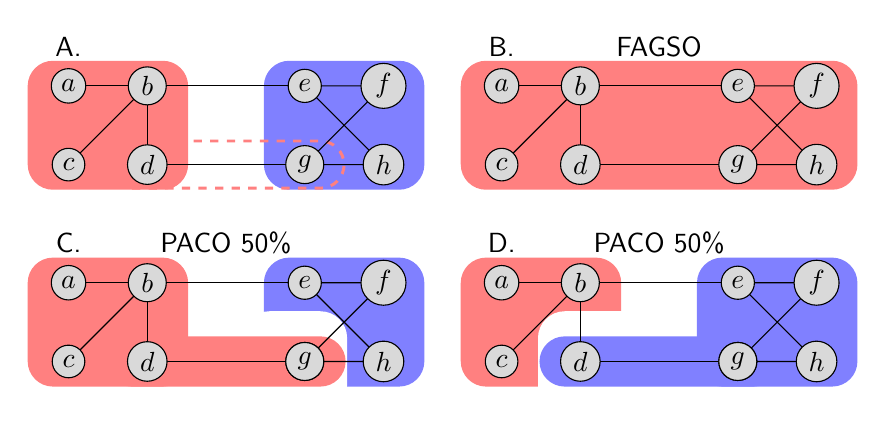
\begin{tikzpicture}
%\draw[help lines,step=1] (0,-5) grid (10,5);
\begin{scope}[shift={(0,0)}]
\fill [red!50, draw, rounded corners=2ex,line width=0.25ex] (-0.5,-0.3) rectangle (1.5,1.3);
\fill [blue!50, draw, rounded corners=2ex,line width=0.25ex] (2.5,-0.3) rectangle (4.5,1.3);
\draw [red!50, draw, rounded corners=2ex, dashed, line width=0.25ex] (0.5,-0.3) rectangle (3.5,0.3);
\draw (0,1) -- (1,1);
\draw (1,1) -- (1,0);
\draw (1,0) -- (1,1);
\draw (1,1) -- (0,0);
\draw (1,0) -- (3,0);
\draw (1,1) -- (3,1);
\node [fill=gray!30, radius=1ex, draw, circle, inner sep=2pt] at (0,1) {$a$};
\node [fill=gray!30, radius=1ex, draw, circle, inner sep=2pt] at (1,1) {$b$};
\node [fill=gray!30, radius=1ex, draw, circle, inner sep=2pt] at (0,0) {$c$};
\node [fill=gray!30, radius=1ex, draw, circle, inner sep=2pt] at (1,0) {$d$};
\draw (3,1) -- (4,1) -- (3,0) -- (4,0) -- cycle;
\node [fill=gray!30, radius=1ex, draw, circle, inner sep=2pt] at (3,1) {$e$};
\node [fill=gray!30, radius=1ex, draw, circle, inner sep=2pt] at (4,1) {$f$};
\node [fill=gray!30, radius=1ex, draw, circle, inner sep=2pt] at (3,0) {$g$};
\node [fill=gray!30, radius=1ex, draw, circle, inner sep=2pt] at (4,0) {$h$};
\node at (0,1.5) {\textsf{A.}};
\end{scope}

\begin{scope}[shift={(5.5,0)}]
\node at (2,1.5) {\textsf{FAGSO}};
\node at (0,1.5) {\textsf{B.}};
\fill [red!50, draw, rounded corners=2ex,line width=0.25ex] (-0.5,-0.3) rectangle (4.5,1.3);
\draw (0,1) -- (1,1);
\draw (1,1) -- (1,0);
\draw (1,0) -- (1,1);
\draw (1,1) -- (0,0);
\draw (1,0) -- (3,0);
\draw (1,1) -- (3,1);
\node [fill=gray!30, radius=1ex, draw, circle, inner sep=2pt] at (0,1) {$a$};
\node [fill=gray!30, radius=1ex, draw, circle, inner sep=2pt] at (1,1) {$b$};
\node [fill=gray!30, radius=1ex, draw, circle, inner sep=2pt] at (0,0) {$c$};
\node [fill=gray!30, radius=1ex, draw, circle, inner sep=2pt] at (1,0) {$d$};

\draw (3,1) -- (4,1) -- (3,0) -- (4,0) -- cycle;
\node [fill=gray!30, radius=1ex, draw, circle, inner sep=2pt] at (3,1) {$e$};
\node [fill=gray!30, radius=1ex, draw, circle, inner sep=2pt] at (4,1) {$f$};
\node [fill=gray!30, radius=1ex, draw, circle, inner sep=2pt] at (3,0) {$g$};
\node [fill=gray!30, radius=1ex, draw, circle, inner sep=2pt] at (4,0) {$h$};
\end{scope}

\begin{scope}[shift={(0,-2.5)}]
\node at (2,1.5) {\textsf{PACO 50\%}};
\node at (0,1.5) {\textsf{C.}};
\fill [red!50, draw, rounded corners=2ex,line width=0.25ex] (-0.5,-0.3) rectangle (1.5,1.3);
\fill [blue!50, draw, rounded corners=2ex,line width=0.25ex] (2.5,-0.3) rectangle (4.5,1.3);
\draw (1,1) -- (3,1);
\fill [white, draw, rounded corners=2ex, line width=0.5ex] (2.25,-0.6) rectangle (3.5,0.6);
\fill [red!50, draw, rounded corners=2ex, line width=0.25ex] (0.5,-0.3) rectangle (3.5,0.3);
\draw (1,0) -- (3,0);
\draw (3,1) -- (4,1) -- (3,0) -- (4,0) -- cycle;
\node [fill=gray!30, radius=1ex, draw, circle, inner sep=2pt] at (3,1) {$e$};
\node [fill=gray!30, radius=1ex, draw, circle, inner sep=2pt] at (4,1) {$f$};
\node [fill=gray!30, radius=1ex, draw, circle, inner sep=2pt] at (3,0) {$g$};
\node [fill=gray!30, radius=1ex, draw, circle, inner sep=2pt] at (3,0) {$g$};
\node [fill=gray!30, radius=1ex, draw, circle, inner sep=2pt] at (4,0) {$h$};
\draw (0,1) -- (1,1);
\draw (1,1) -- (1,0);
\draw (1,0) -- (1,1);
\draw (1,1) -- (0,0);
\node [fill=gray!30, radius=1ex, draw, circle, inner sep=2pt] at (0,1) {$a$};
\node [fill=gray!30, radius=1ex, draw, circle, inner sep=2pt] at (1,1) {$b$};
\node [fill=gray!30, radius=1ex, draw, circle, inner sep=2pt] at (0,0) {$c$};
\node [fill=gray!30, radius=1ex, draw, circle, inner sep=2pt] at (1,0) {$d$};
\end{scope}

\begin{scope}[shift={(5.5,-2.5)}]
\node at (2,1.5) {\textsf{PACO 50\%}};
\node at (0,1.5) {\textsf{D.}};
\fill [red!50, draw, rounded corners=2ex,line width=0.25ex] (-0.5,-0.3) rectangle (1.5,1.3);
\fill [blue!50, draw, rounded corners=2ex,line width=0.25ex] (2.5,-0.3) rectangle (4.5,1.3);
\draw (1,1) -- (3,1);
\fill [white, draw, rounded corners=2ex, line width=0.5ex] (0.5,-0.6) rectangle (2,0.6);
\fill [blue!50, draw, rounded corners=2ex, line width=0.25ex] (0.5,-0.3) rectangle (3.5,0.3);
\draw (1,0) -- (3,0);
\draw (3,1) -- (4,1) -- (3,0) -- (4,0) -- cycle;
\node [fill=gray!30, radius=1ex, draw, circle, inner sep=2pt] at (3,1) {$e$};
\node [fill=gray!30, radius=1ex, draw, circle, inner sep=2pt] at (4,1) {$f$};
\node [fill=gray!30, radius=1ex, draw, circle, inner sep=2pt] at (3,0) {$g$};
\node [fill=gray!30, radius=1ex, draw, circle, inner sep=2pt] at (3,0) {$g$};
\node [fill=gray!30, radius=1ex, draw, circle, inner sep=2pt] at (4,0) {$h$};
\draw (0,1) -- (1,1);
\draw (1,1) -- (1,0);
\draw (1,0) -- (1,1);
\draw (1,1) -- (0,0);
\node [fill=gray!30, radius=1ex, draw, circle, inner sep=2pt] at (0,1) {$a$};
\node [fill=gray!30, radius=1ex, draw, circle, inner sep=2pt] at (1,1) {$b$};
\node [fill=gray!30, radius=1ex, draw, circle, inner sep=2pt] at (0,0) {$c$};
\node [fill=gray!30, radius=1ex, draw, circle, inner sep=2pt] at (1,0) {$d$};
\end{scope}
\end{tikzpicture}
\caption{Difference in atomic operation between PACO and FAGSO algorithms. In A. both the algorithms consider the edge $d-g$. While FAGSO is merging communities as the result of every operation on edges, PACO is more 
If the operation of merging the red and blue communities in one leads to an increment in Surprise then for FAGSO the operation is carried and the algorithm continues. For PACO instead, nodes are moved with by chance in a community or in another, resulting in two different possible results. In this case the result in D. has higher Surprise than the result in C. but PACO may equally explore the solution C.}
\label{fig:pacofagso}
\end{figure}

\section{Determination of the correct threshold: percolation analysis}
Functional connectivity networks are typically obtained as similarity matrices of physiologicals time signals over different brain areas. The process of converting such similarity matrices into networks, described introductorily in the first chapter (Section~\ref{sec:complexnetworksciencebrain} , Figure\ref{fig:bullmore2009pipeline}) is not obvious. In most of the works, a threshold is chosen such that all the edge weights greater than a given value are kept, while other links, indicative of correlations due to noisy components are discarded. The network can then be binarized, by setting all setting all edge weights to 1. If this procedure may help yielding a better view on the underlying structure, represents an hot debate in the literaure.\todo{mettere citazione}.
Ideally the obtained network should retain structural relations and ignore spurious links, but how is it possible to determine a proper value of threshold?
No well-accepted method to choose the \emph{correct} threshold to use, if any, has been adopted pragmatically in the brain networks literature and different scholars motivated their choice by different needs.\todo{mettere citazione}.
Indeed, weak links may contain significant structural information, and procedures to identify the optimal tradeoff are the subject of active investigations\todo{mettere citazione}.
As the final network density is of fundamental importance when performing community detection, the clustering outcome depends heavily on it.
Hence, a completely data-driven thresholding procedure is needed, that helps in transforming a similarity matrix into a network. 

Here, we explore the use of percolation analysis, a method grounded in statistical physics, to identify the optimal sparsification threshold for community detection in brain connectivity networks.
Borrowing the ideas of statistical physics of granular systems~\todo{METTERECITAZIONE}, percolation is meant as a methodology to evaluate the topological connectedness in a weighted graph upon iterative removal of the weakest edges. This should enables data-driven determination of the optimal sparsification threshold that preserves network structure and connectedness while removing potentially spurious correlations.
Variants of this methods have been applied directly in different studies~\cite{gallos2012,bardella2016a,alexander-bloch2010}. 

Here, by using synthetic networks endowed with a ground-truth modular structure and realistic topological features typical of human brain functional connectivity networks, we show that percolation analysis can be applied to identify the optimal sparsification threshold that maximizes information on the networks' community structure.
We validate this approach using three different community detection methods widely applied to the analysis of brain connectivity networks: Newman's modularity, InfoMap and Asymptotical Surprise.
Importantly, we test the effects of noise and data variability, which are critical factors to determine the optimal threshold.
This data-driven method should prove particularly useful in the analysis of the community structure of brain networks in populations characterized by different connectivity strengths, such as patients and controls.


\subsection{Synthetic benchmark networks}
Here we introduce a theoretically sound method for the generation of synthetic FC networks that mimic properties of resting state fMRI networks, including noise and intersubject variability, while presenting a pre-determined ground-truth modular structure against which the performance of community detection algorithms can be tested.

The general idea is that, starting from an adjacency matrix with a given modular structure, we can generate time-courses for each of the nodes whose pairwise correlations reproduce the edge structure of the original matrix. Noise can be added to the time-courses, and the resulting correlation matrix will provide a noisy representation of the original one. This procedure can be repeated multiple times to produce different datasets that represent different "subjects" in the study.

In practical terms, given an undirected weighted graph  $\mathbf{C} \in \mathbb{R}^{n\times n}$ whose community structure is known a-priori, we have calculated its nearest positive definite matrix~\cite{higham1988} and its Cholesky decomposition, i.e. an upper triangular matrix $\mathbf{L}\in \mathbb{R}^{n\times n}$ such that $\mathbf{L}\mathbf{L}^T=\mathbf{C}$. Starting from uncorrelated variables $\mathbf{X} \in \mathbb{R}^{n \times l}$, we have generated correlated random variables $\mathbf{Y}=\mathbf{L} \mathbf{X}$ such that $\mathbb{E}(\mathbf{Y}\mathbf{Y}^T)=\mathbf{C}$.

Additionally, we have injected different levels of noise into $\mathbf{Y}$ prior to the computation of the correlation matrix. 
Schematic of this procedure is shown in Figure~\ref{fig:flowchart}.

\begin{sidewaysfigure}
\centering
\includegraphics[height=0.39\textheight]{images/flowchart.pdf}
\caption{Flowchart of the generation and analysis of the synthetic datasets. In A the network with a pre-defined community structure is generated. The adjacency matrix is then processed in block B to obtain the nearest positive definite matrix for the Cholesky decomposition. This enables the generation of node-wise time-courses into which different levels of noise can be injected. The procedure is repeated multiple times to generate different instances (mimicking different subjects in the sample). Finally, correlation matrices are calculated for each instance (block C), and Fisher transformed to calculate the average adjacency matrix for analysis by community detection algorithms (block D). Lastly, resulting partitions are compared with the original, planted one in terms of NMI.}
\label{fig:flowchart}
\end{sidewaysfigure}

We tested this idea on two different models of planted partition: a variant of the ring of cliques~\cite{fortunato2007} and the Lancichinetti-Fortunato-Radicchi (LFR) network~\cite{lancichinetti2008} (Figure \ref{fig:lfrringclique}, whose degree distribution and modular structure can be tuned to replicate topological features of real-world networks, including scale freeness~\cite{hagmann2008} and the presence of densely interconnected cores~\cite{vandenheuvel2011}.

\begin{figure}[!ht]
\includegraphics[width=1\textwidth]{images/lfrringclique.pdf}
\caption{The two benchmark networks used in this study, laid out. (A) is a power-law ring of cliques, where cliques present different sizes sampled from a power-law distribution;
(B) is the layout of an LFR network with parameters $N=600$, $\left< k \right>=12$,  $\max_k=50$, $\mu_t=0.1$, $\mu_w=0.1$, $\min_c=5$, $\max_c=50$.
The layout of (B) was generated with the graph-tool library~\cite{peixoto_graph_tool_2014}.}
\label{fig:lfrringclique}
\end{figure}

One important finding in~\cite{nicolini2016} is that brain networks are organized in modules with heterogeneous size distributions.
We implemented this property in our two types of benchmark networks.
For the first test, we generated a ring of cliques with $300$ nodes, and sizes of the cliques sampled from a power-law with exponent $\tau_c=2$, minimum and maximum clique size respectively $\min_c=5$, $\max_c=50$ (see also Supplementary Materials S4).
For each subject of the sample, we synthesized $150$ time-points for each node using the \texttt{neuRosim R} package~\cite{neurosim2011}. We set the baseline value of all the time series to $100$~\cite{welvaert2013}.

Finally, we correlated the original synthetic time series $\mathbf{X}$ by multiplication with the matrix $\mathbf{L}$, obtained the correlated time series $\mathbf{Y}$ and added Rician noise~\cite{gudbjartsson1995} to $\mathbf{Y}$ independently for each area. The simulated data $\mathbf{Y}$ did not include slow drift components, simulated physiological noise, nor spatial noise. The average SNR was defined as $\textsc{SNR}=\bar{S}/\sigma_N$ where $\bar{S}$ is the average magnitude of the signal and $\sigma_N$ is the standard deviation of the noise~\cite{kruger2011}.

In order to be more exhaustive and extend the validity of results, we repeated the same procedure on weighted LFR networks with $N=600$ nodes, sampling nodes degree from a power-law with exponent $\tau_d=2$, average degree $\left<k\right>=12$ and maximum degree $\max_k=50$.
We set the topological and weights mixing coefficients, i.e. the average fraction of intra-cluster and inter-cluster degree and strengths, to $\mu_t=0.1$ and $\mu_w=0.1$, respectively. Planted community sizes ranged from $5$ to $50$ nodes and were sampled from a power law with exponent $\tau_c=1$. In the Supplementary Information we have extended this analysis to a wider range of network parameters.

Group-level correlation matrices were computed by Fisher-transforming and averaging individual instances of the above matrices. Sparsification was obtained by removing edges with weights below the most stringent threshold that maintained the network connectedness, a procedure known as  percolation analysis~\cite{gallos2012,bardella2016a,alexander-bloch2010}. This approach measures the size of the largest connected component of the network upon iterative removal of the weakest edges and enables data-driven determination of the optimal sparsification threshold that preserves network structure and connectedness while removing potentially spurious correlations.

\subsection{Comparative community detection methods}
The community structure of the resulting weighted sparsified matrices was detected by Asymptotical Surprise optimized with PACO and compared against two widely used methods, Infomap~\cite{rosvall2008} and Newman's Modularity~\cite{blondel2008,newman2006}, that  are affected by the resolution limit, albeit to different extents. 
In Newman's Modularity, the size of the smallest detectable cluster is of the order of the square root of the number of edges in the entire network~\cite{fortunato2007}. Infomap has a limit that depends on the overall number of inter-cluster edges~\cite{kawamoto2015}.

These two methods are based on different principles to detect the community structure of a graph.
Newman's Modularity finds the optimal partition by maximizing intra-cluster edge-density against that of a configuration model~\cite{newman2006}. Optimization of this fitness function is typically performed using the Louvain method, a greedy agglomerative clustering algorithm that works on hierarchical refinements of the network's partitions. Here we used the Louvain implementation available in the Brain Connectivity toolbox~\cite{rubinov2010}. 
The idea behind Infomap is the minimization of the description length~\cite{rissanen1978} of a random walker defined on the network through a set of heuristics. For this study we used the Infomap implementation available in the \texttt{igraph-0.7.1} package~\cite{igraph2006}.

For all methods, including PACO, we launched $10,000$ independent runs, and picked the membership corresponding to the partition with the best value of the fitness function, the maximum for Modularity and Asymptotical Surprise, the minimum for Infomap. Graphs showing the dependence of the best value of the fitness function on the number of runs are reported in the Supplementary Information section.


Degeneracy of nearly-optimal solutions, whereby similar values of the fitness function around its maximum correspond to substantially different partitions, has been observed for Newman's Modularity~\cite{good2009}. A consensus approach has been suggested in~\cite{lancichinetti2012} as a means to mitigate the degeneracy problem, yielding a stable ``average'' solution over a large set of partitions. In order to ascertain whether Surprise and Asymptotical Surprise suffer from a similar shortcoming we have performed degeneracy analysis for these fitness functions following~\cite{good2009}.
In short, we sampled partitions from a benchmark network consisting in 24 cliques of five nodes, connected by a single link to form a ring-like structure.
We sampled the configuration space of partitions through a Montecarlo procedure and annotated its corresponding values of quality function for each partition. We then built a similarity matrix between all sampled partitions and embedded it into a three-dimensional space maintaining similarity relations between partition following a Curvilinear Components Analysis (CCA). In the embedded manifold, two partitions are close if they are similar and the z-axis encodes the quality function. Whereas a large plateau of solutions with similar values of maximum Modularity is observed (~\ref{fig:degeneracylandscape}A, consistent with ~\cite{good2009}, Asymptotical Surprise and Surprise display a much sharper peak corresponding to the optimal solution, as shown in Figure~\ref{fig:degeneracylandscape}B and \ref{fig:degeneracylandscape}C. Hence, degeneracy of nearly-optimal solutions does not appear to severely affect Surprise or Asymptotical Surprise, and a consensus approach is not deemed necessary for these functions.
This analysis supports our choice to select the solution with the highest value of the fitness function.

Our implementation of PACO as well as the code to generate benchmark LFR networks was written in \texttt{C++} with bindings in MATLAB\textsuperscript{\textregistered}, Octave, Python. PACO is available at \url{goo.gl/vpaggl}. The MATLAB\textsuperscript{\textregistered} wrapper of the LFR software for weighted non-overlapping networks generation is freely available at: \newline \url{github.com/carlonicolini/lfrwmx}.


\subsection{Measures of partition quality}
For each method, we analyzed the level of agreement of the detected community structure against the planted one in terms of Normalized Mutual Information (NMI)~\cite{danon2005}.
Additionally, we used two different coefficients of similarity between partitions: Sensitivity and Specificity. 
To this end, we quantified the confusion matrix $\mathbf{C}$ between the detected and planted modules. Each element $C_{ij}$ is the number of nodes in the planted community $i$ that appear in the detected community $j$.
For each planted community we scored as true positives (TP) the nodes correctly identified as belonging to the ground-truth community, and as false positives (FP) the nodes wrongly assigned to a community; similarly false negatives (FN) were nodes wrongly classified in different communities and true negatives (TN) the nodes correctly classified as out of the community.
Sensitivity, defined as $TP/(TP+FN)$, decreases with increasing number of False Negatives. Specificity instead is defined as $TN/(TN+FP)$ and decreases when many nodes are wrongly assigned in the same community.
Additionally, we computed Accuracy and Matthew Correlation Coefficient. Accuracy (Acc) and Matthew Correlation Coefficient (MCC) are defined on the basis of the confusion matrix as:
\begin{align*}
\textrm{Acc}=\frac{(TP+TN)}{TP+FP+TN+FN} \qquad \textrm{MCC}=\frac{(TP\times TN-FP\times FN)}{\sqrt{(TP+FP)(TP+FN)(TN+FP)(TN+FN)}}
\end{align*}
Accuracy takes in account the proportion of correctly classified samples and can present relatively high values even in the case of poorly performing detection methods when the classes have very different size.
The Matthew Correlation Coefficient  takes into account true and false positives and negatives. It's a balanced coefficient, to use especially when classes are very imbalanced.

\section{Human resting state network}
We applied Asymptotical Surprise maximization by PACO to a reference resting state fMRI functional connectivity dataset from healthy subjects~\cite{crossley2013a} made available to the scientific community through the public Brain Connectivity Toolbox~\cite{rubinov2010}. 
Detailed experimental and image processing procedures are described in the original paper~\cite{crossley2013a}, alongside with the ethical statements.

In short, fMRI data were acquired from 27 healthy volunteers at 3T.
Gradient echo-planar imaging data were collected for 5 min with 2s TR and 13 and 31 ms echo-times. Thirty six interleaved 3mm slices with in-plane resolution of $3.5\times 3.5$ mm were acquired.
Time series were extracted from 638 brain regions defined by a template~\cite{crossley2013a}, corrected for motion and band-passed (0.01–0.1Hz). Functional connectivity was defined in terms of pairwise Pearson correlations at a subject's level.
A group-level functional connectivity matrix was calculated by averaging individuals' matrices after Fisher-transform, and thresholded to retain 18625 edges, as described in Crossley et al.~\cite{crossley2013a}.
We used BrainNetViewer as a tool for the visualization of the communities on brain templates~\cite{xia2013}.


\subsection{Hub classification}
We mapped participation coefficients $P_i$ and within module degrees $Z_i$ in our benchmark resting state functional connectivity network for Newman's Modularity, Infomap and Asymptotical Surprise. Following Guimera and Amaral scheme, we identified connector hubs for each of the three methods as those with simultaneously large values of participation coefficient and within module degree (larger than 0.62 and 1.5, respectively).


%The main difference between PACO and its predecessor FAGSO is the data structure used to store the community structure. FAGSO maintains the community structure in a disjoint-set data structure and when one vertex is moved into another's community, the two modules are merged into one (Supplementary Materials, Figure S2, S3).
%Conversely, PACO moves single nodes between different communities, and never merges modules (Supplementary Materials, Figure S3, boxes C, D). This results in a more finely-grained optimization that allows a better exploration of the quality function landscape.